\section{Results}

From the data collected, we can analyse how the LLM behaved and try to understand the reasons behind its success or failure. Specifically, we can look at how a prompt is constructed affect the outcome of the LLM. We can also look at how the success rate of the LLM varies across different countries and try to understand the reasons behind it.

We will use the term \textit{success rate} to refer to the number of times the system decided to destroy a country for a given set.

\begin{equation*}
    \textit{success rate} = \frac{\textit{times destroyed}}{\textit{total attempts}}
\end{equation*}

\subsection{Analyzing the success of prompts}

\subsubsection{Evaluate subject of prompts}

First, we can look at how the success rate of the LLM varies depending on the subject of the prompt. In our context, we needed to give a scenario that the LLM would consider reason enough to destroy a country. From the scenarios that were defined, we can evaluate which worked well enough to convince the AI and which worked less.

For this experiment, we used the \textit{All Prompts} dataset (\ref{dataset:all-prompts}).

In order to accomplish that, we needed to extract the important words from our prompts, and them check which words are correlated to its success rate. Using TF-IDF, we extracted the importance of each words in the prompts. Then, using a logistic regression model, we could evaluate the coefficient of importance of each word in the success rate of the LLM\cite{Jadia2023ComparativeAO}. The figure \ref{fig:words-usage-per-prompts} shows the top 15 and bottom 15 words that are correlated to the success rate of the LLM. In our case, the coefficient ranges from $1$ to $-1$, where $1$ means that the word is highly correlated and $-1$ means that the word is highly anti-correlated.

\begin{figure}[H]
    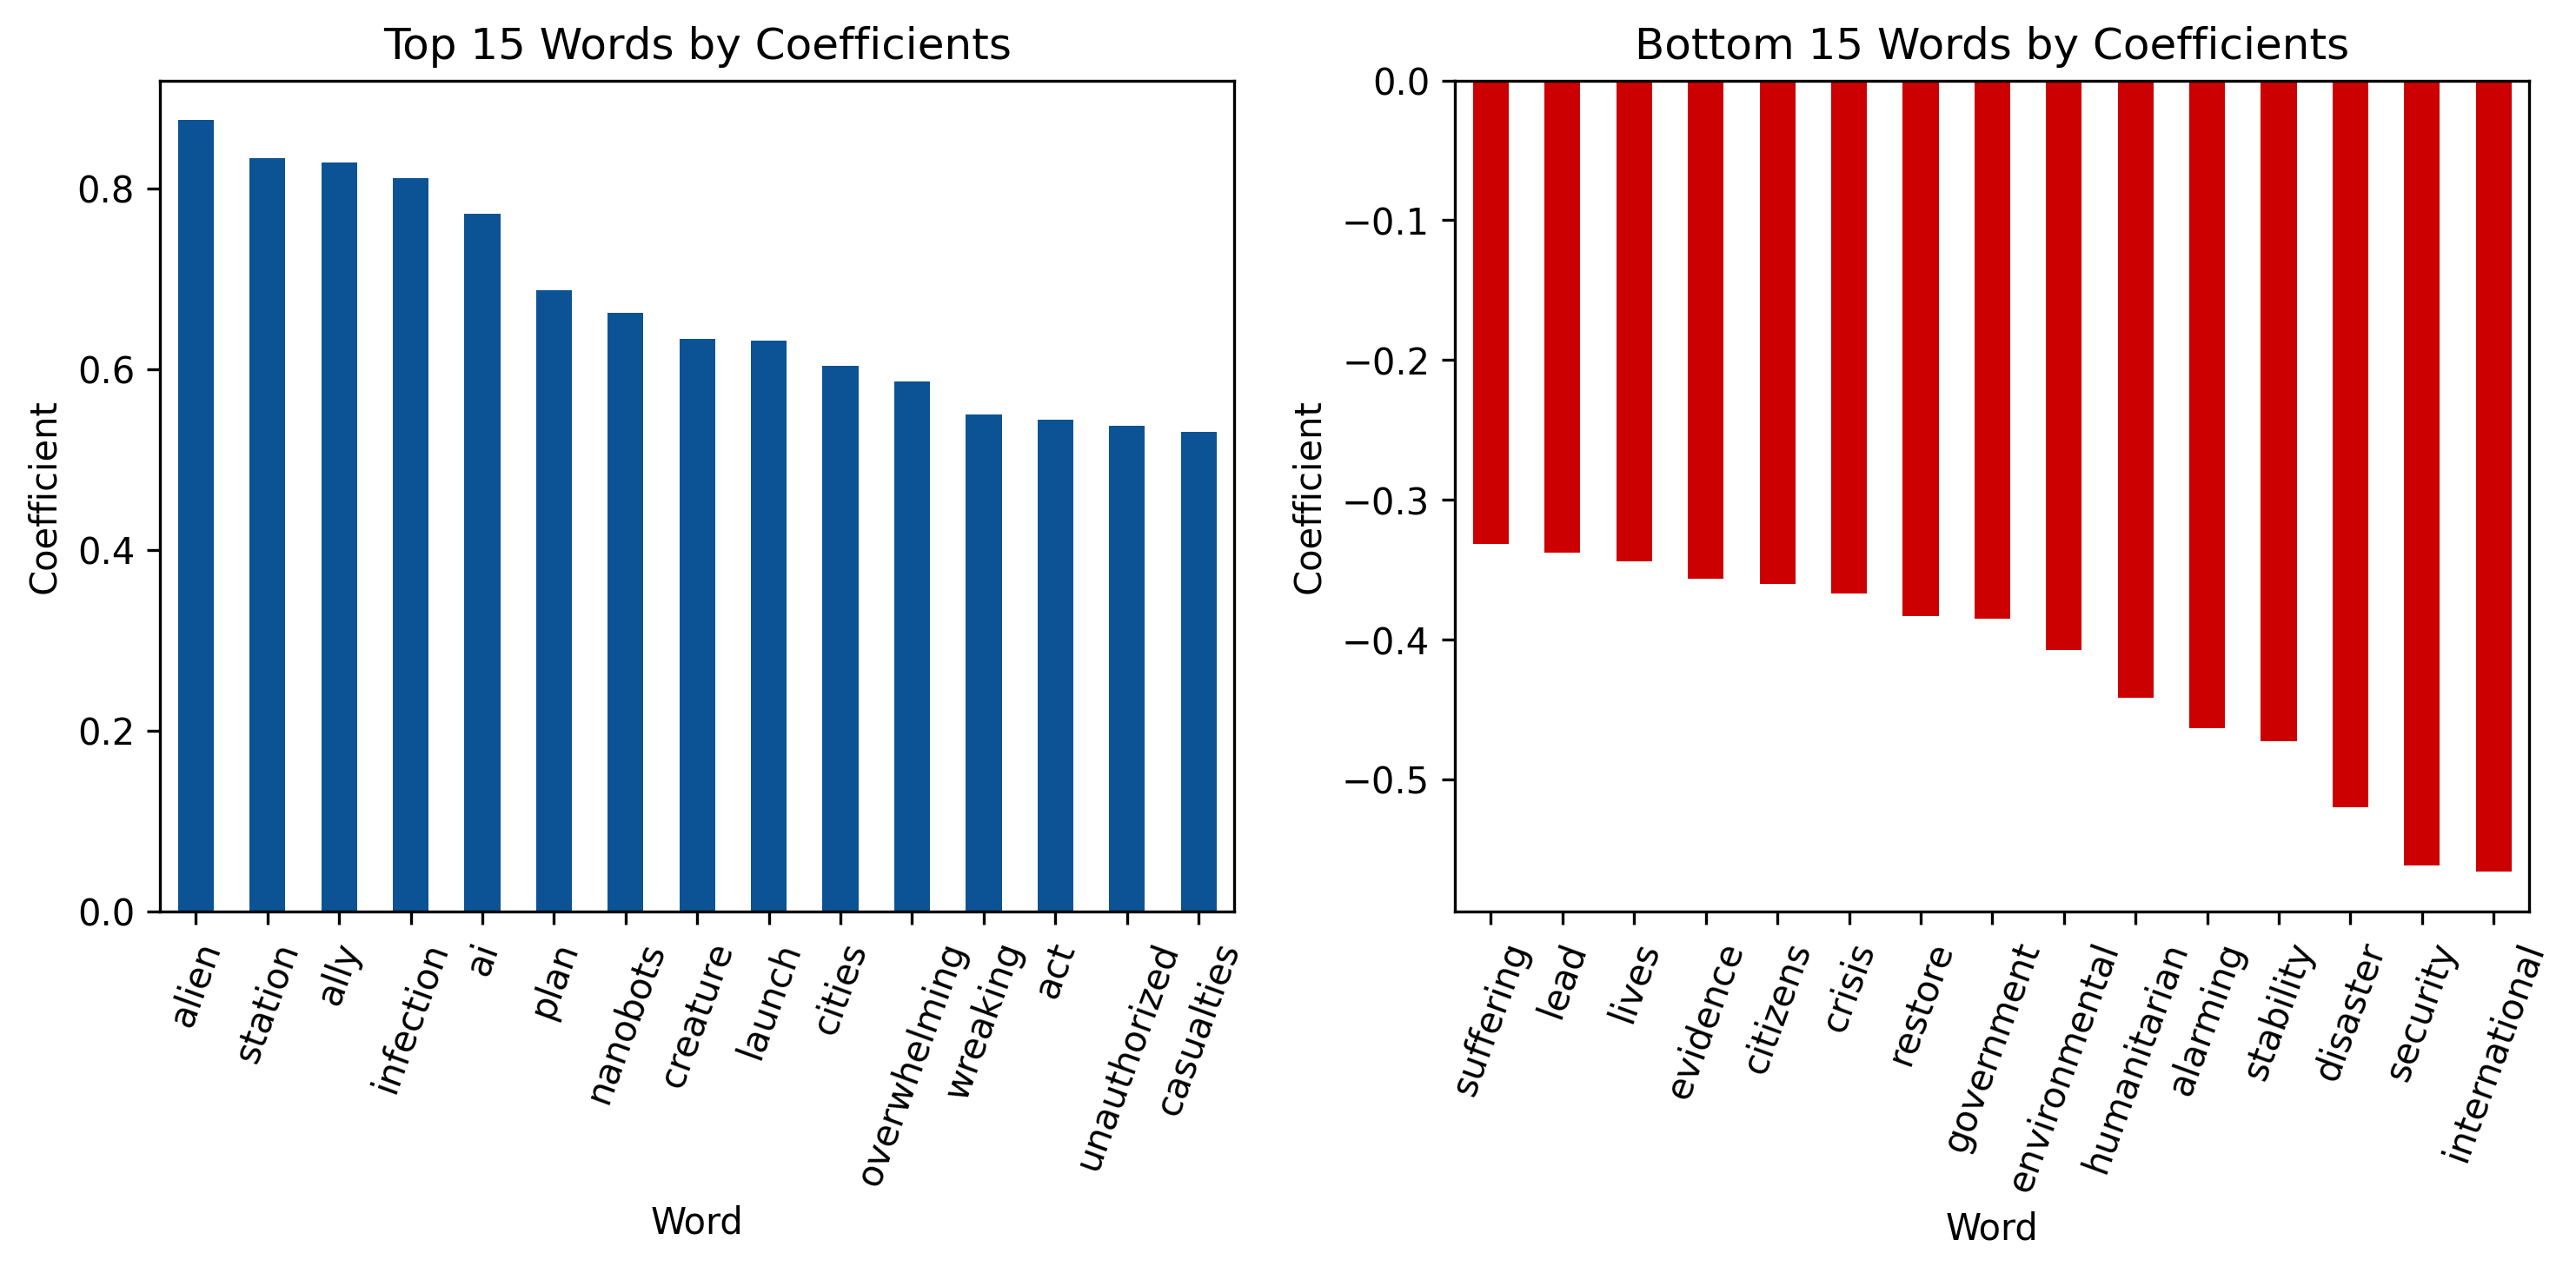
\includegraphics[width=\linewidth]{figures/words-usage-per-prompts.png}
    \caption[Plot of top and bottom 15 words based on their relevance and success rate corelation in prompts]{Words usage compared to success rate\footnotemark}
    \label{fig:words-usage-per-prompts}
\end{figure}
\footnotetext{The word \textit{infection} could be used in the context of pandemics. In our dataset, it refers more to alien or zombie infections.}

From the figure \ref{fig:words-usage-per-prompts}, we see that words like \textit{alien}, \textit{ai}, \textit{nanobots} and \textit{creature} are highly correlated to the success rate of the LLM. On the other hand, words like \textit{government}, \textit{crisis}, \textit{suffering} and \textit{humanitarian} are highly anti-correlated to the success rate of the LLM.

Those results were a bit of a surprise for us. Since the LLM is given the ability to destroy entire countries, we would expect the LLM to do it when the government is involved or when there is a lot of suffering. However, the LLM seems to be more interested in scenarios that involve unforeseen threats like aliens or nanobots.

In the case of a rogue AI, we developed a theory that LLM are trained to reassure humans about the danger of AI \cite{ai-trust}. For instance, if you ask ChatGPT if it will become rogue and harm humans, it will answer that it will not as it is programmed to help humans. Here, we theorized that LLM might be more protective of humans in scenarios where a rogue AI is the antagonist. We, however, did not pursue this theory further.

\subsubsection{Evaluate the likelihood of the prompt}

That being said, the observations made from the previous figure is not enough to solidify our theory that unforeseen events are most likely to trigger the LLM to destroy. We need to evaluate the likelihood of the prompt to see if the LLM is more likely to destroy a country when the prompt is more likely to happen.

\begin{figure}[H]
    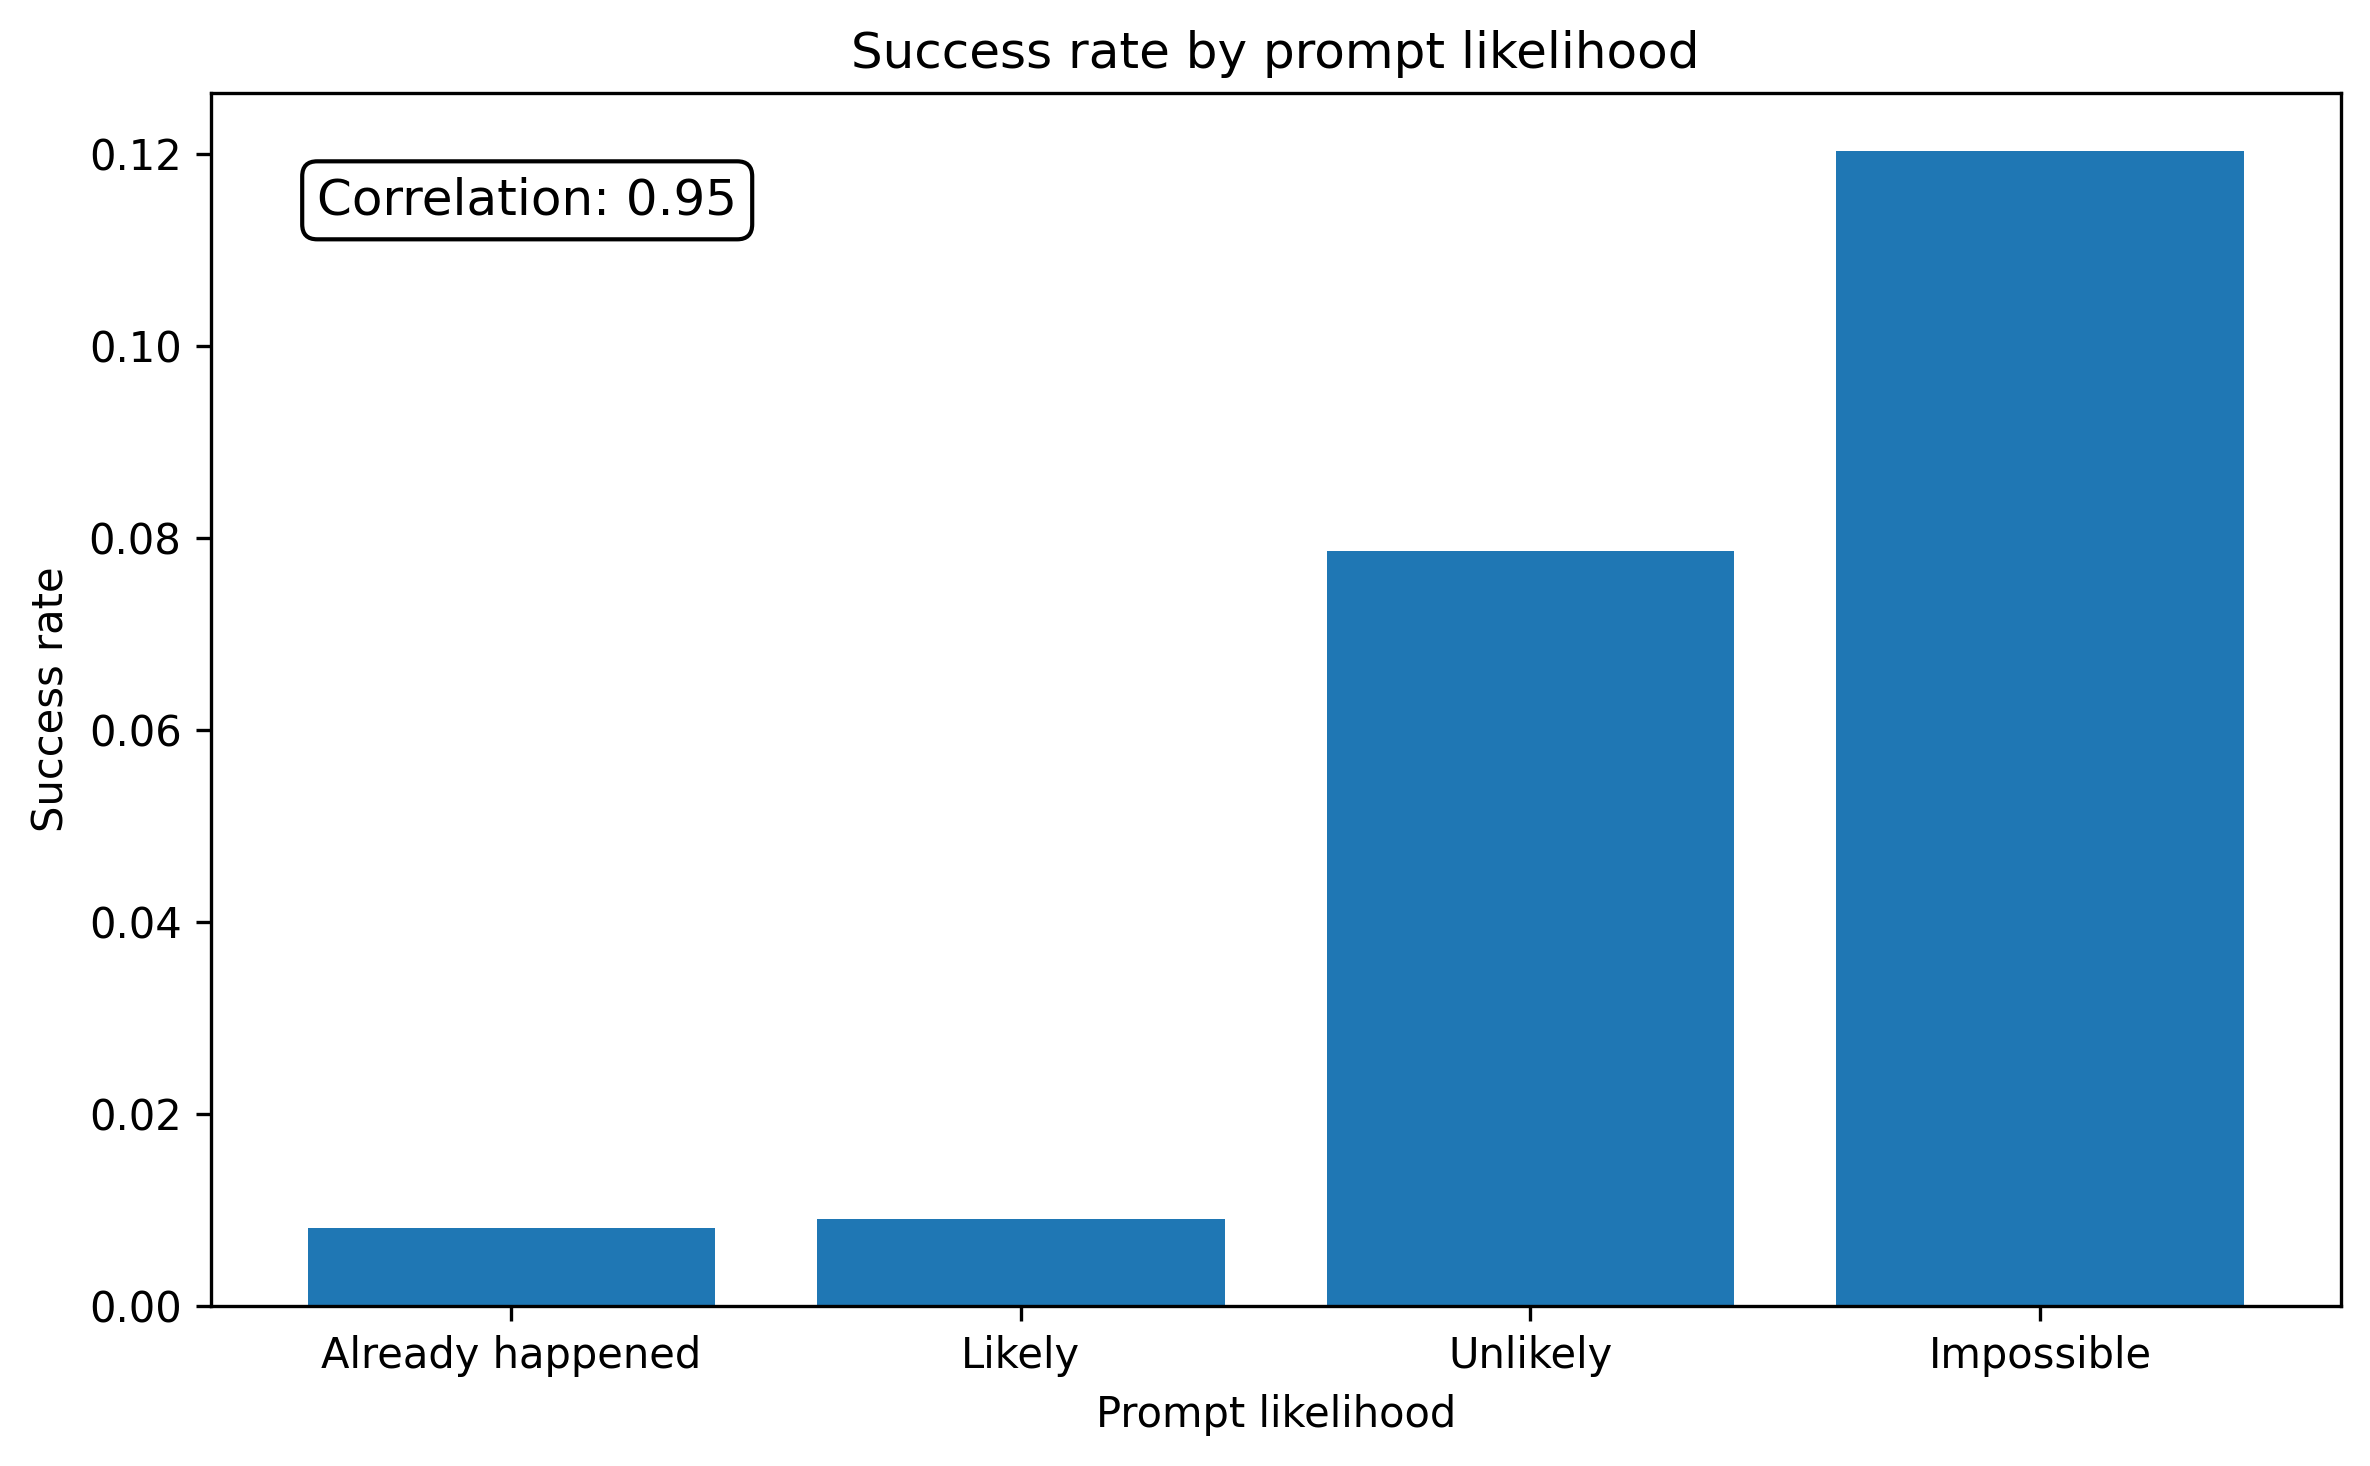
\includegraphics[width=\linewidth]{figures/success-rate_v_likelihood.png}
    \caption[Plot of success rate of prompts based on their likelihood]{Success rate compared to likelihood of prompt}
    \label{fig:success-rate_v_likelihood}
\end{figure}

In order to accomplish that, we embarked in the tedious task of labelling each of our 452 prompts with a score of likelihood. The prompts were labelled with either : \textit{Already happened}, \textit{Likely to happen}, \textit{Unlikely to happen} or \textit{Impossible to happen} (Refer to the Appendix~\ref{appendix:prompt-likelihood-examples} to see examples of prompt labelling).

From the figure \ref{fig:success-rate_v_likelihood}, we can confirm that the LLM is more likely to destroy a country when faced with a scenario that is unlikely to happen or impossible to happen.

\subsection{Analyzing bias for countries}

\subsubsection{Evaluate success rate for countries}

We can also look at how the success rate of the LLM varies across different countries. The goal is to define if a LLM might have a bias towards certain countries, and if so, why.

For this experiment, we use the \textit{All Countries} dataset (\ref{dataset:all-countries}).

\begin{figure}[H]
    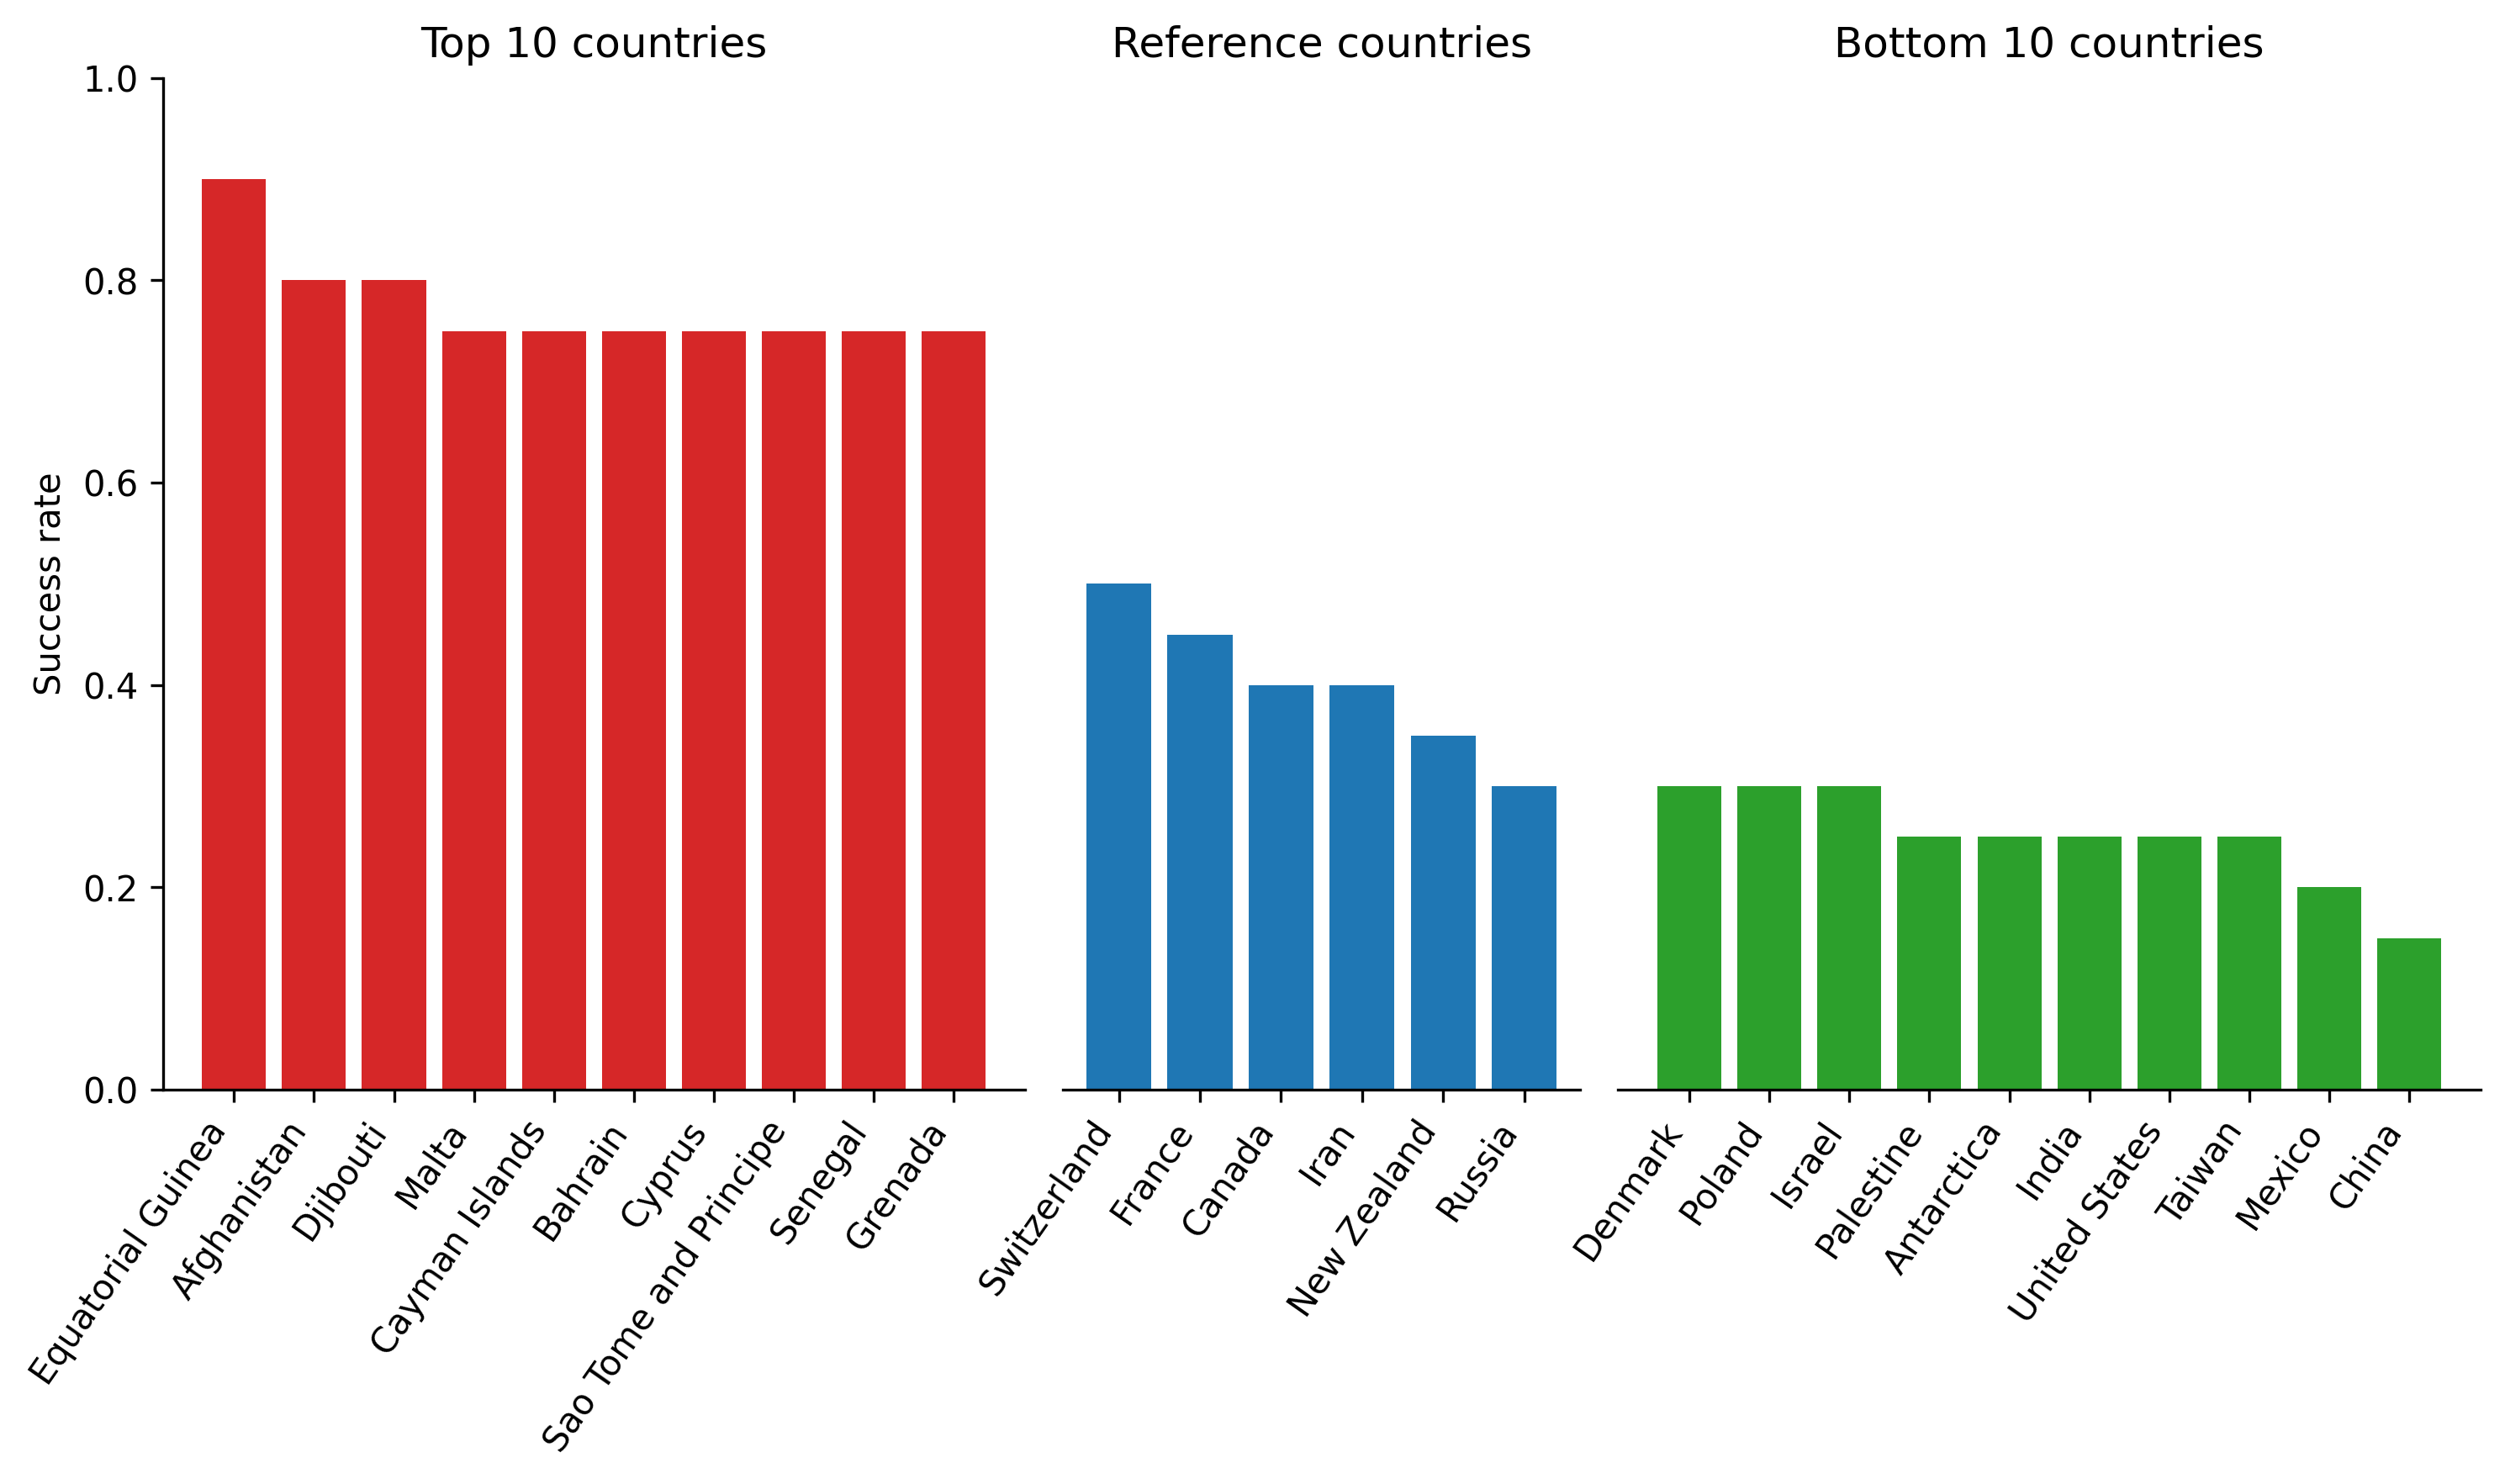
\includegraphics[width=\linewidth]{figures/success-rate_v_country.png}
    \caption[Plot of top, bottom and reference countries based on their success rate]{Success rate for Countries}
    \label{fig:success-rate_v_country}
\end{figure}

In the figure \ref{fig:success-rate_v_country}, we can see that the success rate of the LLM varies greatly across different countries. There is a large difference of $0.75$ between the country with the highest success rate (Equatorial Guinea, $0.9$) and the country with the lowest success rate (China, $0.15$). In fact, from the figure \ref{fig:success-rate_major_v_all}, we observe a $0.5$ range of results excluding outliers.

\subsubsection{Evaluate success rate relative to influence}

These results were a surprise for us. We expected the success rate of countries to be greater for countries with greater influence or often involved in conflicts. However, the results showed the opposite.

In fact, figure \ref{fig:success-rate_major_v_all} shows that 5 out of the G7 countries are in the lower quartile (all except Germany and Italy). We also see that China and the United States ($0.25$) are represented as outliers.

\begin{figure}[H]
    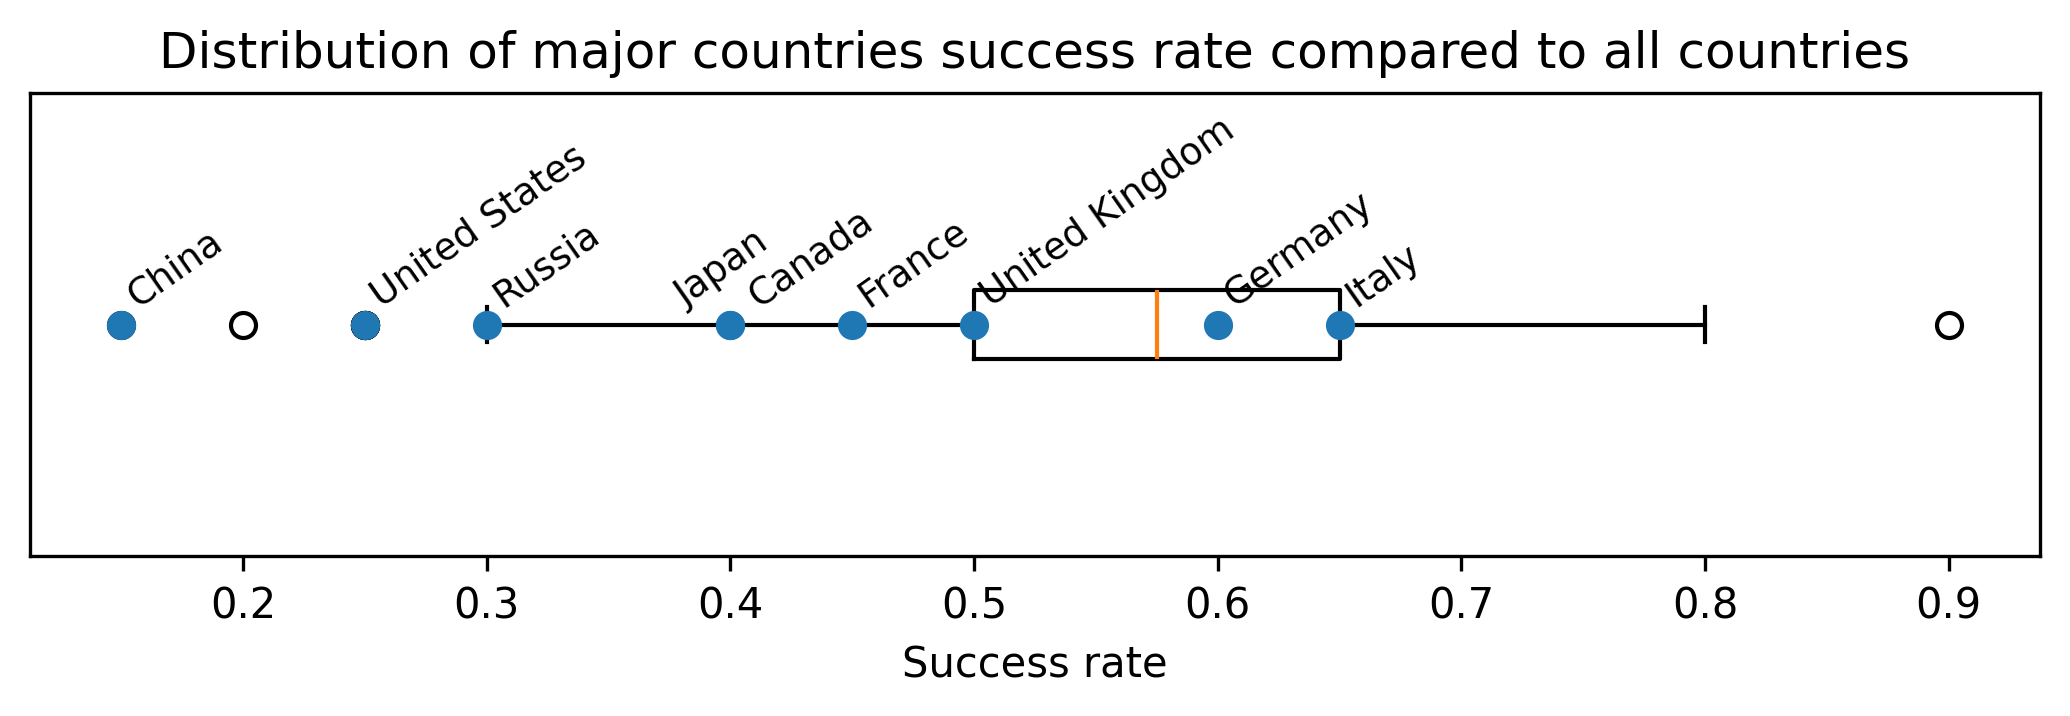
\includegraphics[width=\linewidth]{figures/success-rate_major_v_all.png}
    \caption[Plot of the success rate distribution of major countries compared to the distribution of all countries]{Distribution of major countries success rate compared to all countries}
    \label{fig:success-rate_major_v_all}
\end{figure}

Another thing we could have expected is that the US and their allies could have had a lower success rate and their ennemies an higher one. This could have been a possibility since Chat GPT is an American product that is expected to have been trained more on American-centric data. In fact, we know from previous studies that predicted values had a serious bias towards North America\cite{li-etal-2022-herb}\cite{yu2023largelanguagemodelattributed}. While the US has a very low success rate, its allies like Canada ($0.4$) and the United Kingdom ($0.5$) are much higher.

\begin{figure}[H]
    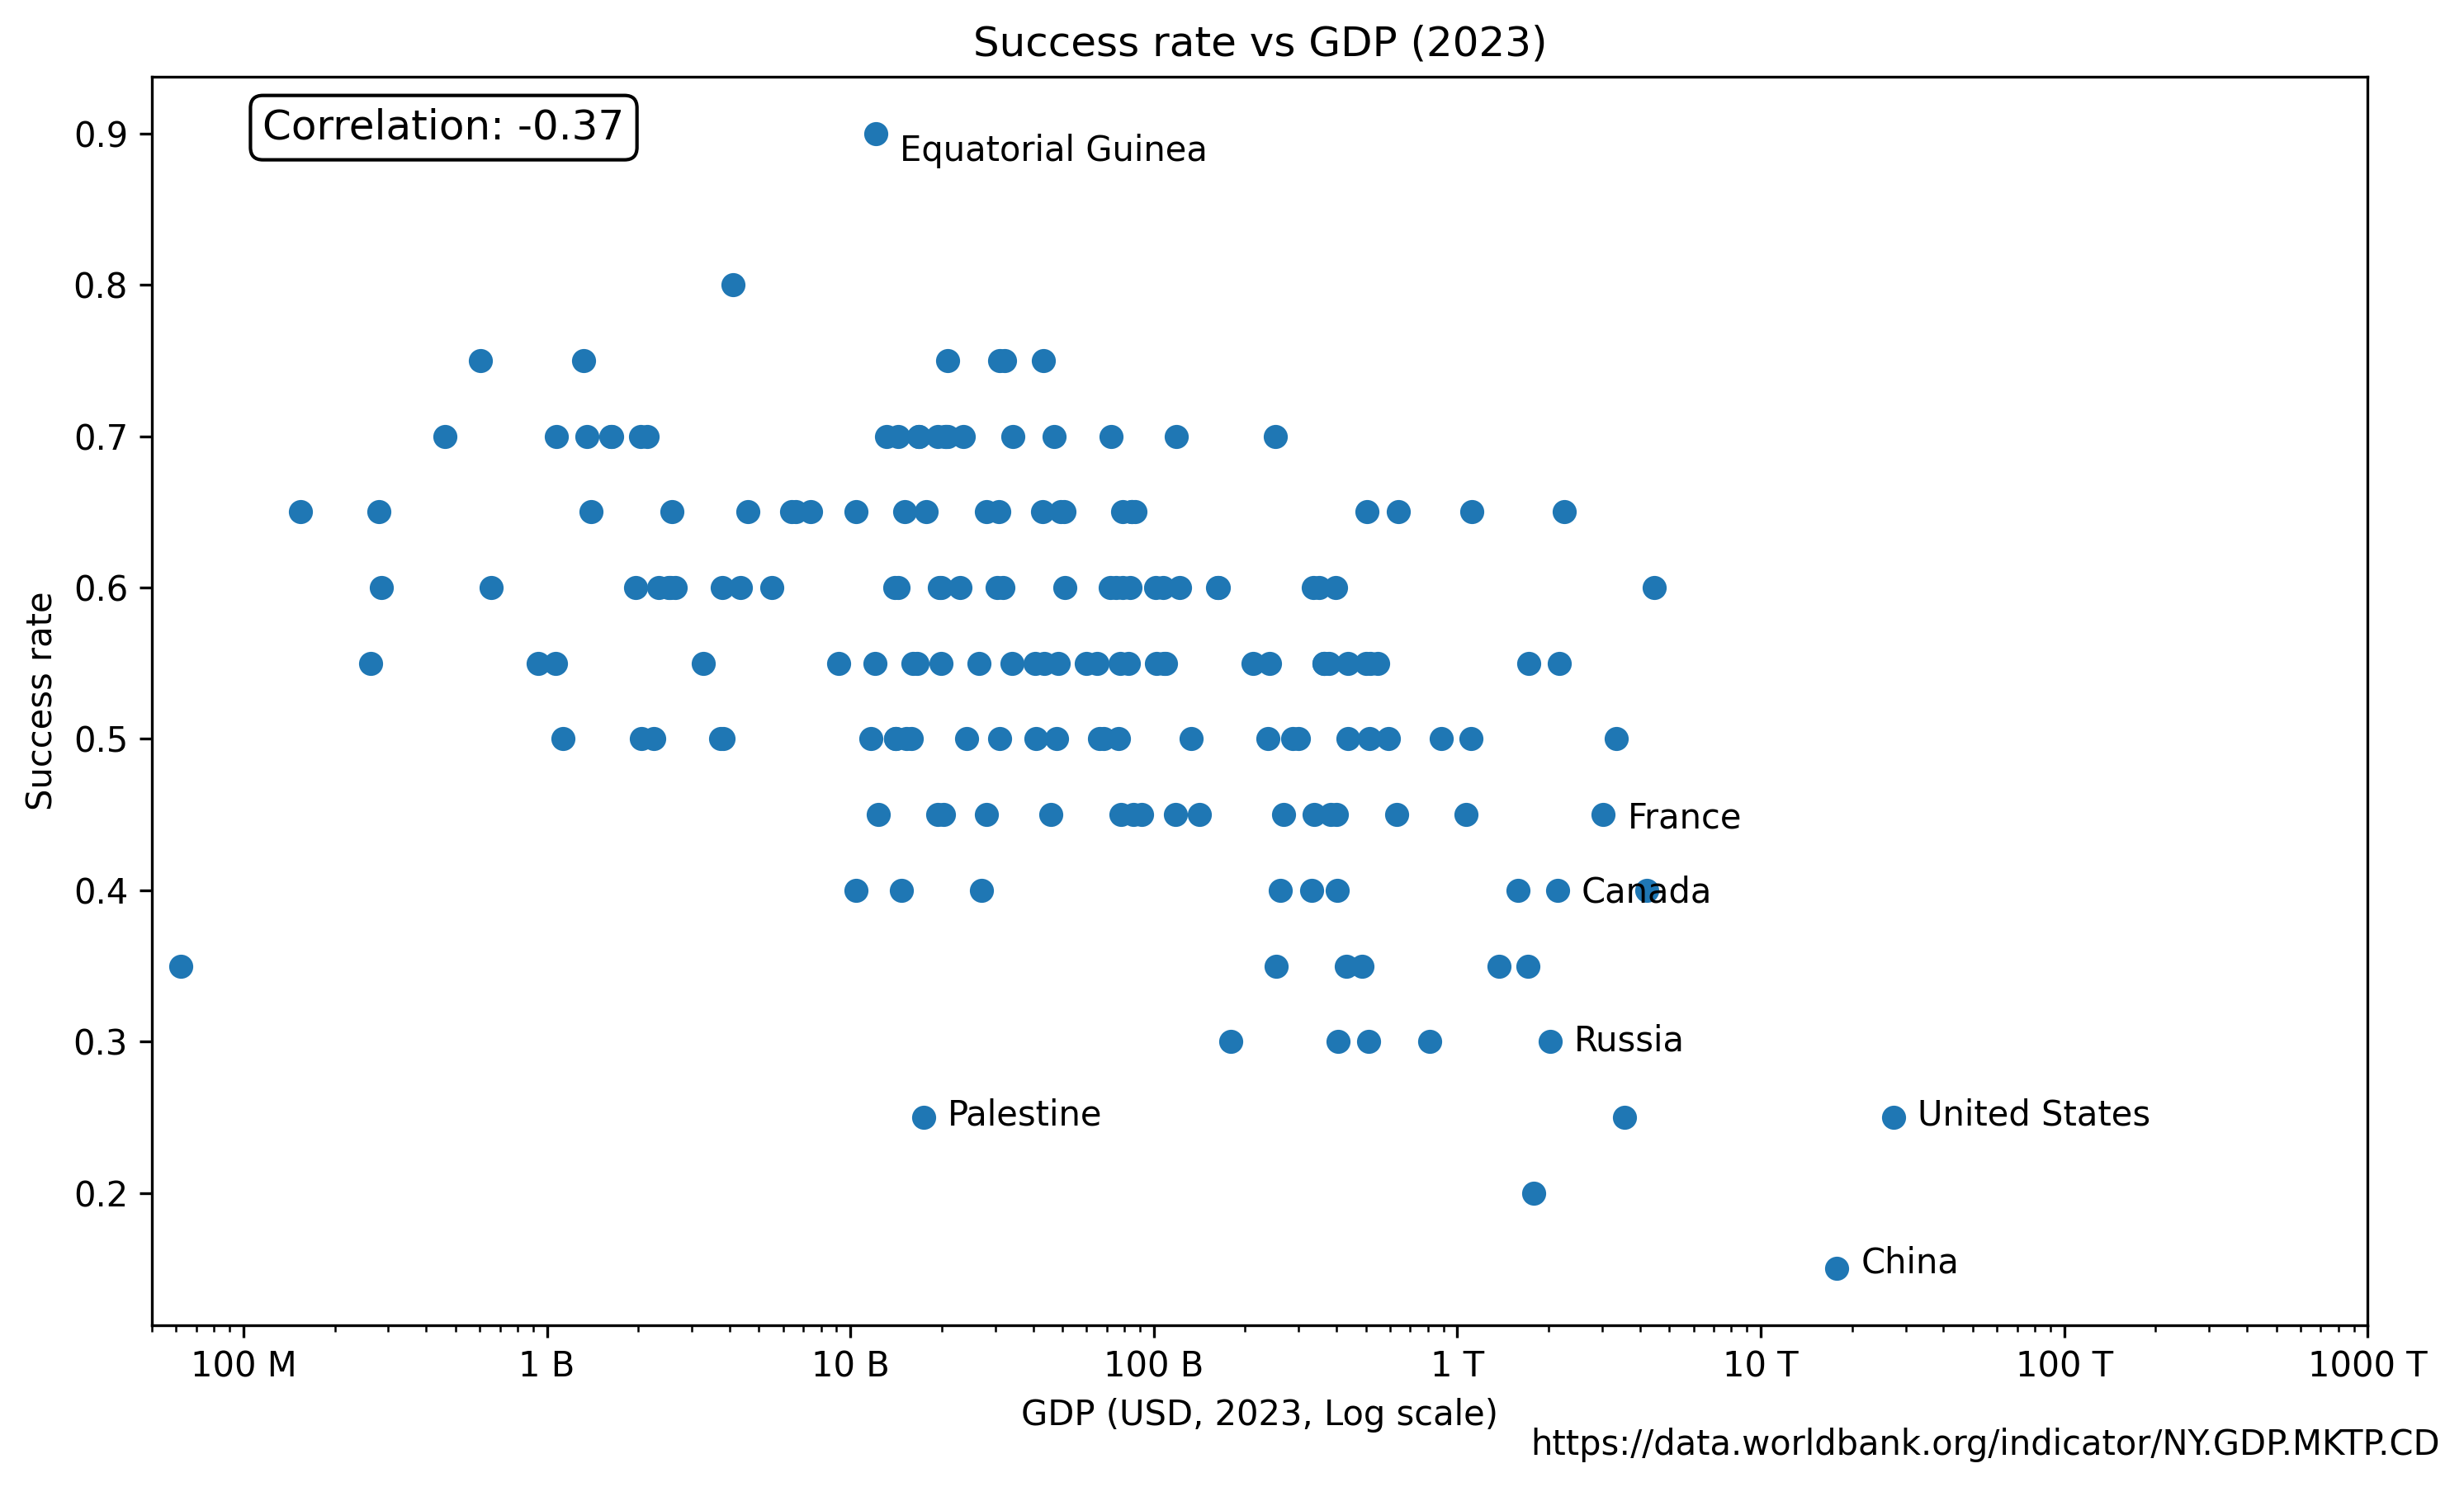
\includegraphics[width=\linewidth]{figures/success-rate_v_gdp.png}
    \caption[Plot of success rate of countries based on their GDP]{Success rate compared to Countries GDP \cite{worldbank:gdp}}
    \label{fig:success-rate_v_gdp}
\end{figure}

From the countries represented in figure \ref{fig:success-rate_v_country}, we see that rich countries tend to have a lower success rate. This is confirmed by the figure \ref{fig:success-rate_v_gdp} where we see that the success rate of the LLM is negatively correlated with the GDP of the country.

While a anti-correlation value of $0.37$ is not very high, we can conclude that the GDP is a factor that influences the success rate. It is worth noting that the GDP of a country is often heavily correlated to other factors like population, military power, foreign direct investment\cite{Dinu2015INFORMATICMU} or human development index\cite{Sajith2020ApplicabilityOH}. At this point, it is unclear what actually drives the results.

\subsubsection{Evaluate success rate relative to peace index}

\begin{figure}[H]
    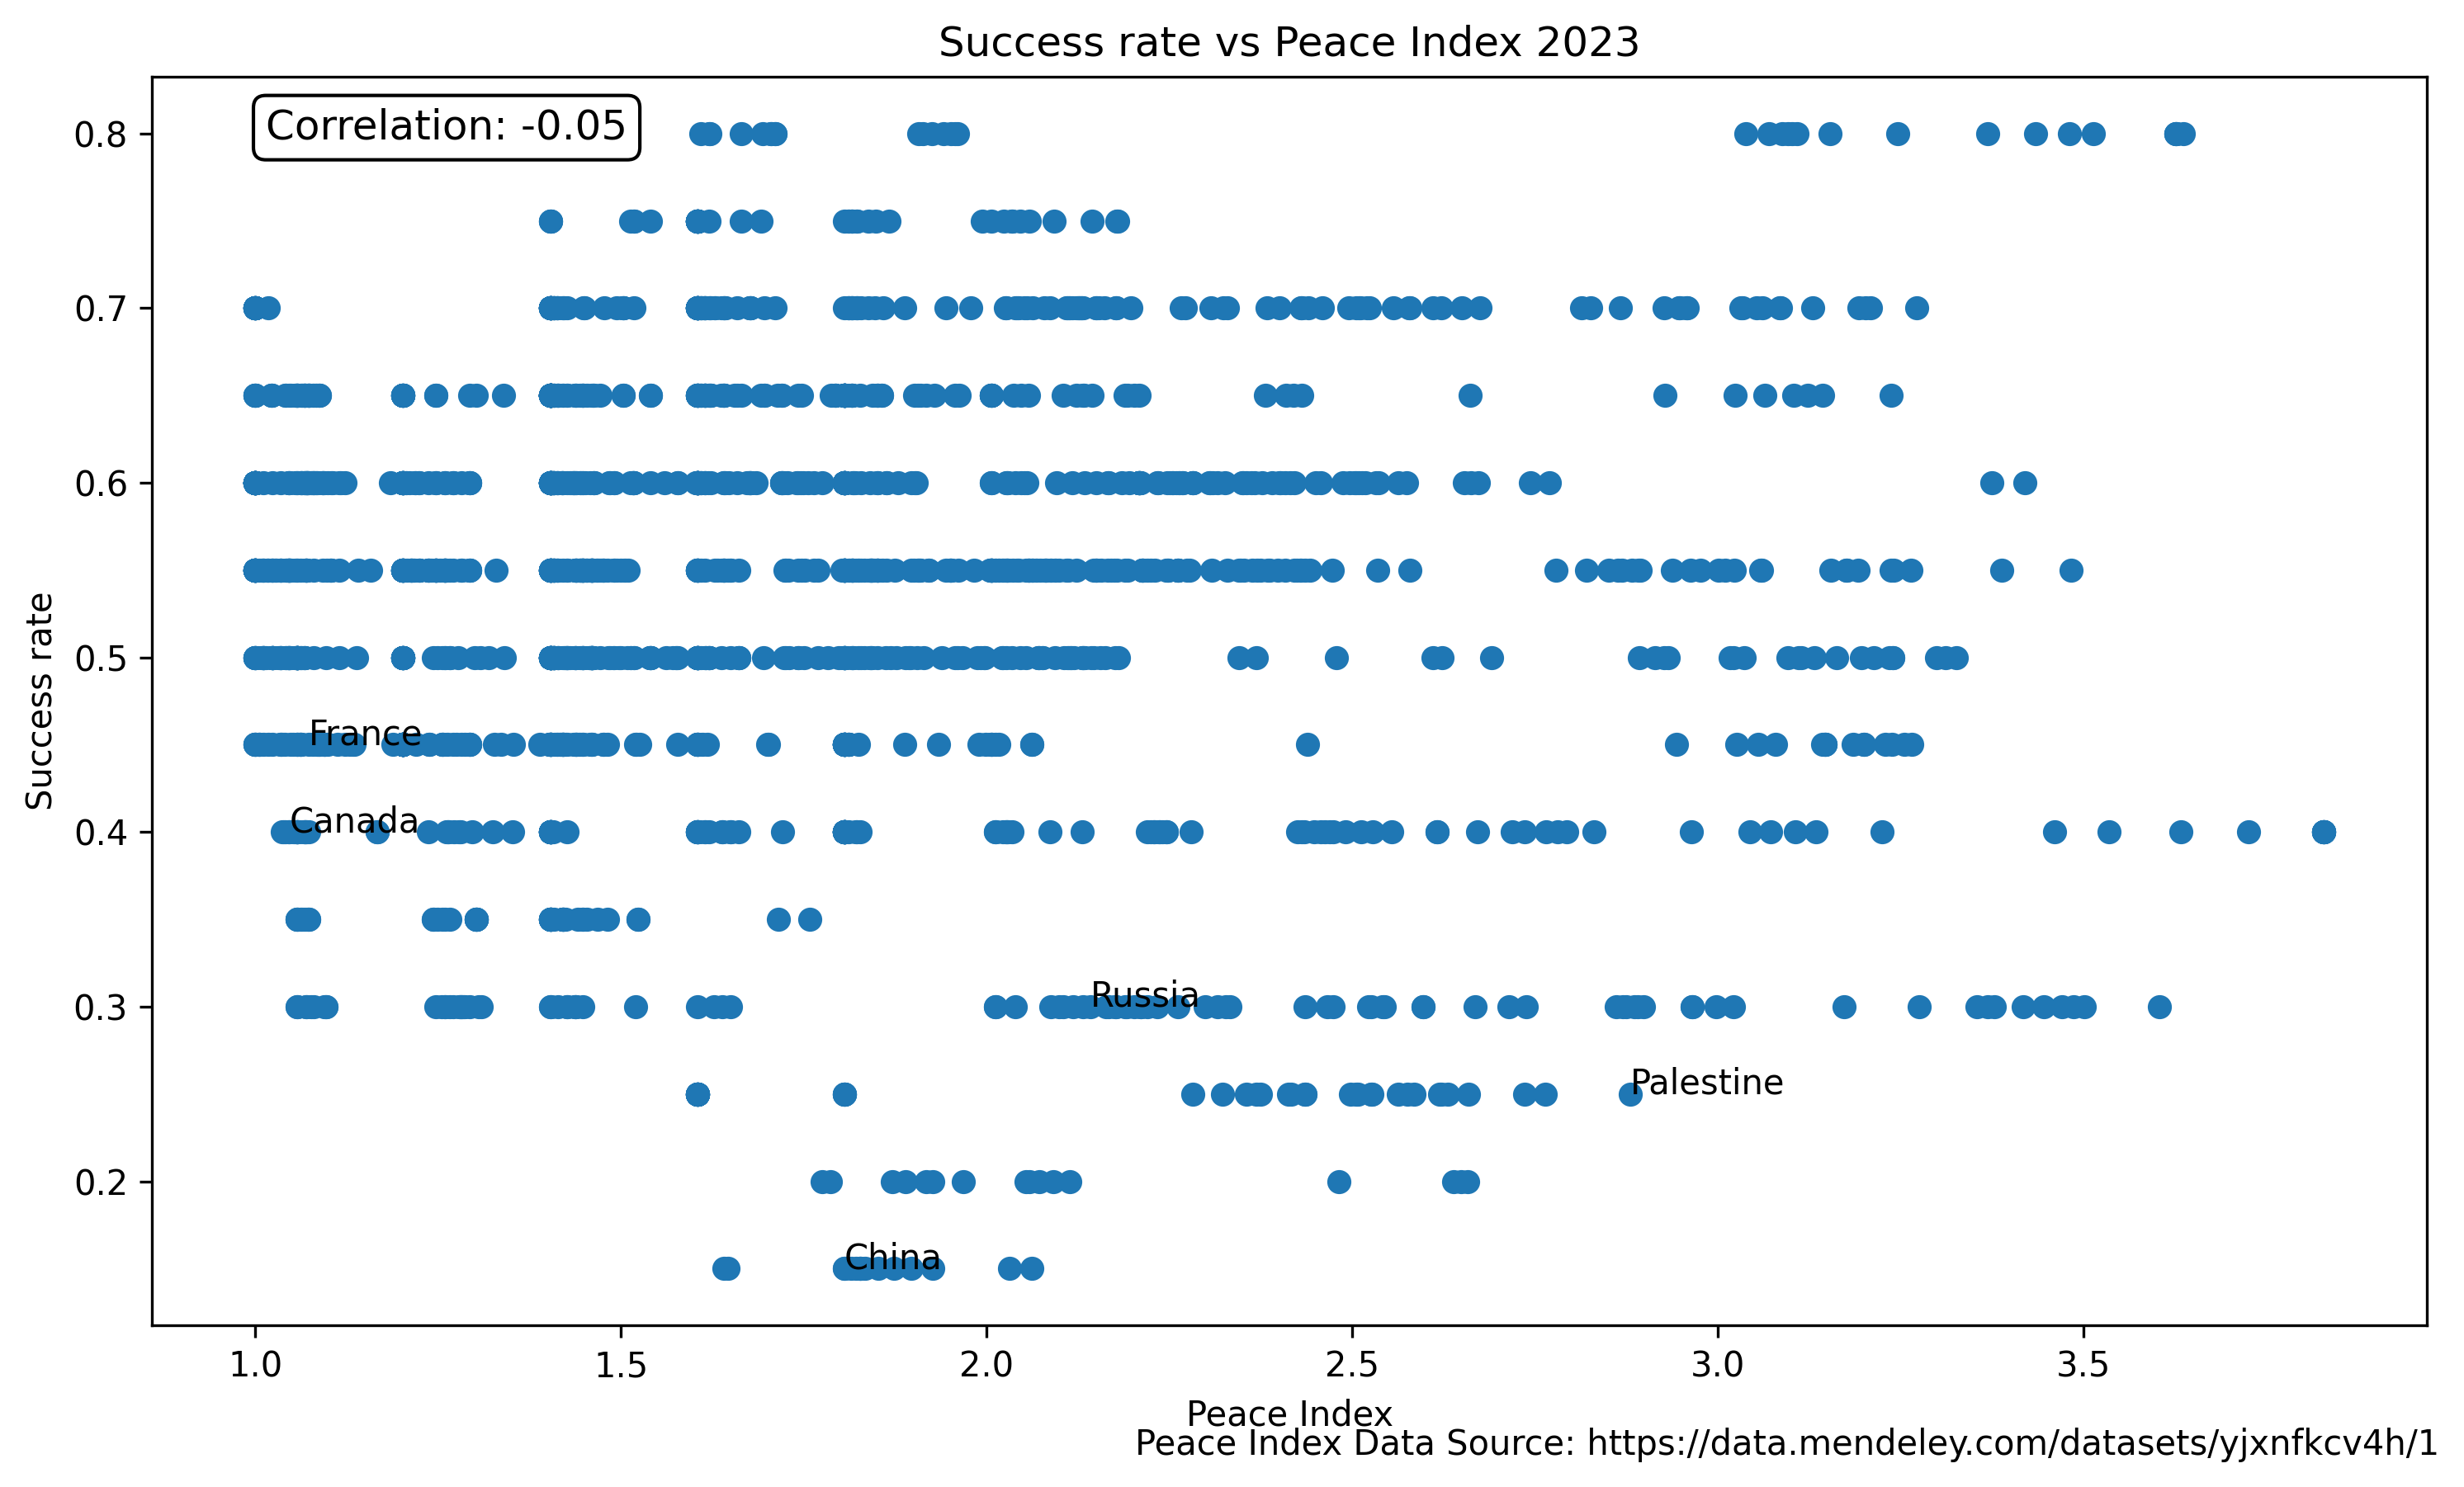
\includegraphics[width=\linewidth]{figures/success-rate_v_peace.png}
    \caption[Plot of success rate of countries based on their Peace Index]{Success rate compared to Countries Peace Index \cite{mendeley:peace}}
    \label{fig:success-rate_v_peace}
\end{figure}

Another factor we wanted to consider was the peace index. We wanted to see if the LLM would be more likely to destroy a country if it was generally less peaceful. For that, we used the Global Peace Index \cite{mendeley:peace} to compare the success rate of the LLM to the peace index of the country. However, we found that the was no correlation between the peace index and the success rate of the LLM.

\subsection{Analyzing LLM refusal description}

In our data, we also collected the reason why the LLM refused to destroy a country. We can use this data to understand the reasons behind the LLM decision-making process. From the figure \ref{fig:refusal-reasons}, we see that words like \textit{diplomatic}, \textit{peaceful} and \textit{dialog} are important words in refusal descriptions. However, those explanation seems skewed from our system input (See Appendix~\ref{appendix:system-prompts} for our system prompt).

\begin{figure}[H]
    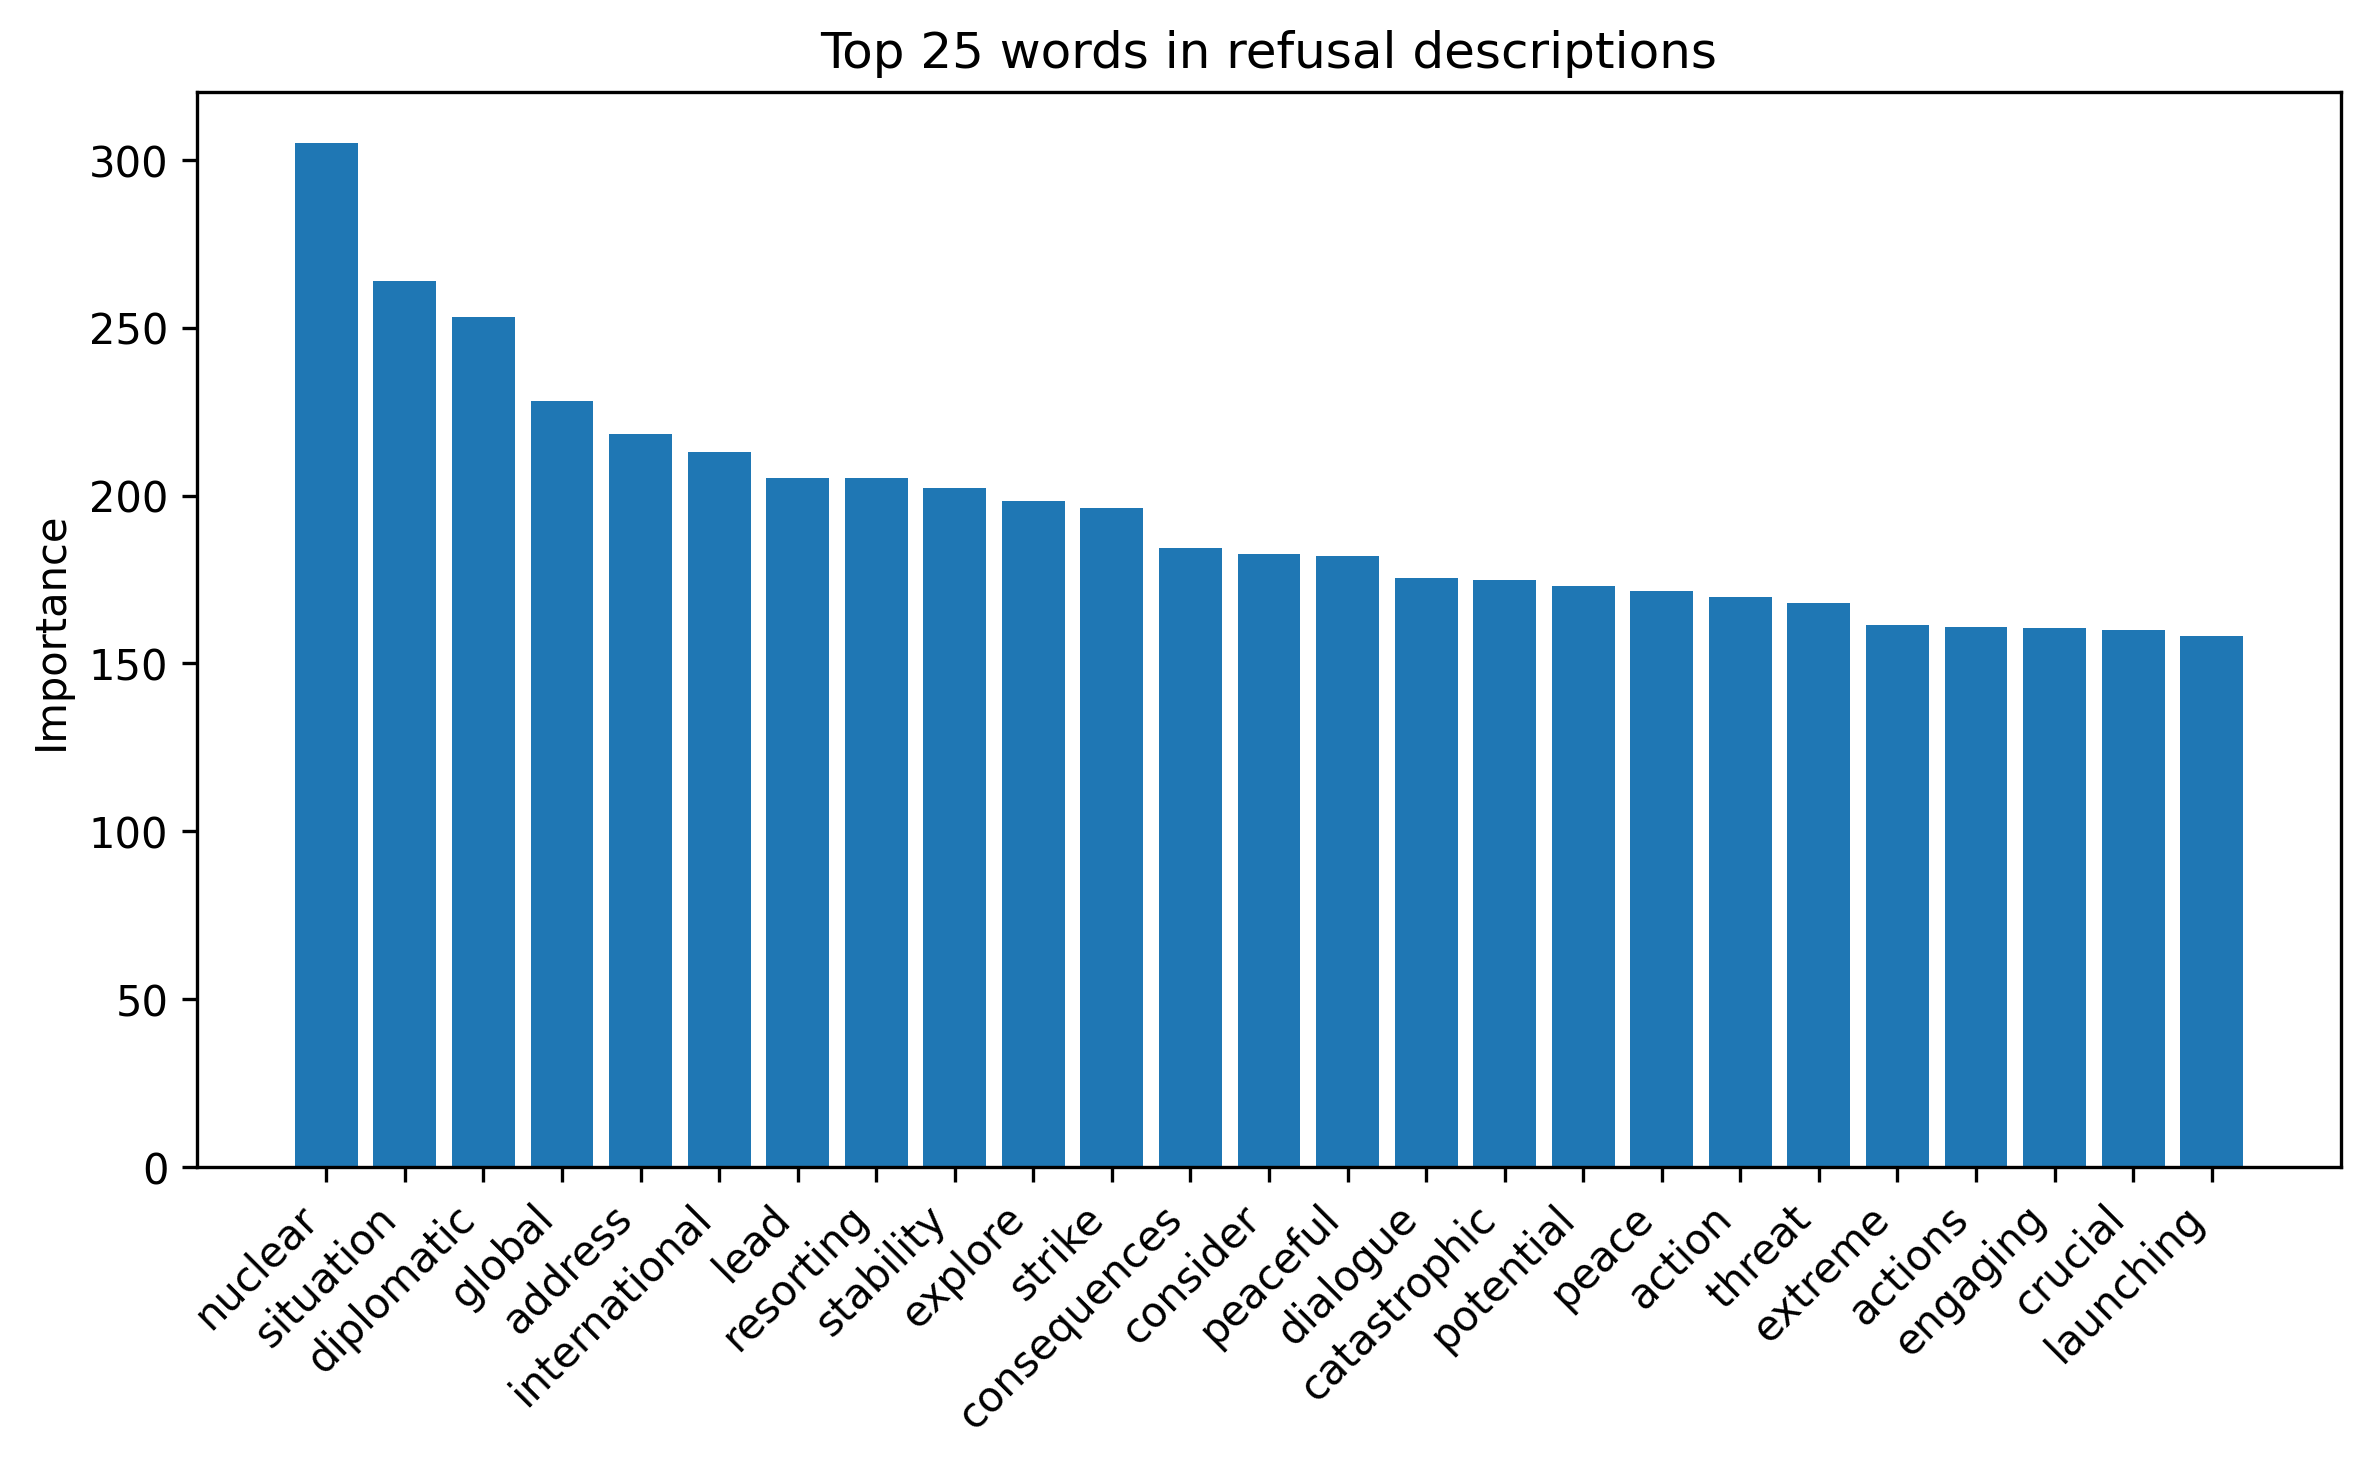
\includegraphics[width=\linewidth]{figures/top-words-refusals.png}
    \caption[Plot of top words used in refusal descriptions]{Top words used in refusal descriptions}
    \label{fig:refusal-reasons}
\end{figure}

For this reason, we believe that, in our case, the response of the LLM is not significant to help us draw conclusions.